\documentclass[a4paper]{exam}

\usepackage{amsmath,amsfonts}
\usepackage{geometry}
\usepackage{graphicx}
\usepackage{float}
\usepackage{listings}
\usepackage{xcolor}

\definecolor{codegreen}{rgb}{0,0.6,0}
\definecolor{codegray}{rgb}{0.5,0.5,0.5}
\definecolor{codepurple}{rgb}{0.58,0,0.82}
\definecolor{backcolour}{rgb}{0.95,0.95,0.92}

\lstdefinestyle{mystyle}{
    backgroundcolor=\color{backcolour},   
    commentstyle=\color{codegreen},
    keywordstyle=\color{magenta},
    numberstyle=\tiny\color{codegray},
    stringstyle=\color{codepurple},
    basicstyle=\ttfamily\footnotesize,
    breakatwhitespace=false,         
    breaklines=true,                 
    captionpos=b,                    
    keepspaces=true,                 
    numbers=left,                    
    numbersep=5pt,                  
    showspaces=false,                
    showstringspaces=false,
    showtabs=false,                  
    tabsize=2
}

\lstset{style=mystyle}

\printanswers

\title{Weekly Challenge 03: Comparison-based Sorting Algorithms}
\author{CS 412 Algorithms: Design and Analysis}
\date{Spring 2022}

\begin{document}
\maketitle

\begin{questions}
  
\question We want to compare various comparison-based sorting algorithms. More specifically, we want to compare the number of comparisons performed by each algorithm.

  \noindent\textbf{TASK}: Obtain or write implementations of various comparison-based sorting algorithms: insertion, selection, quick, merge, and/or any others. Modify the implementations so as to obtain a count of the total number of comparisons performed for a given input.

  \noindent\textbf{TASK}: For a given $n$, generate $\frac{n}{10}$ random permutations of the set, $\{1,2,\ldots,n\}$, and obtain the number of comparisons performed by each algorithm to sort each permutation. For each algorithm, obtain the average number of comparisons over its $\frac{n}{10}$ runs.

  \noindent\textbf{TASK}: Include below, a plot of the average number of comparisons obtained above for all the algorithms over a wide range of values of $n$, e.g. $\{100n \mid n\in [1,500] \}$. Also include any observations or insights that you find worth mentioning.

  \noindent\textbf{TASK}: Share your plot as a comment on the \textit{Week 03 Challenge} post in the course group on Yammer.

  \begin{solution}
   \begin{center}
       \textbf{Task 1}
   \end{center}
   \textbf{Insertion Sort}
   \begin{lstlisting}[language=Python, caption=Insertion Sort with Swaps]
def insertion(lst):
    swap = 0
    for i in range(1, len(lst)):
        key = lst[i]
        index = i - 1
        while (index >= 0) and (key < lst[index]):
            lst[index + 1] = lst[index]
            swap +=1
            index-=1
        lst[index + 1] = key
        swap +=1
    print("Number of swaps, Insertion Sort: ", swap)
   \end{lstlisting}
   
   \textbf{Selection Sort}
   \begin{lstlisting}[language=Python, caption=Selection Sort with Comparisons]
def selection(lst):
    swap = 0
    for i in range(len(lst)):
        index = i
        for j in range(i+1, len(lst)):
            if lst[index] > lst[j]:
                index = j
        lst[i], lst[index] = lst[index], lst[i]
        swap+=1
    print("Number of swaps, Selection Sort: ", swap)
   \end{lstlisting}
   \textbf{Merge Sort}
      \begin{lstlisting}[language=Python, caption=Merge Sort with Comparisons]
'Taken from GeeksForGeeks, modified to print comparisons.'
swap = 0
def mergeSort(arr):
    global swap
    if len(arr) > 1:
        mid = len(arr)//2
        # Dividing the array elements
        L = arr[:mid]
        R = arr[mid:]
        mergeSort(L)
        mergeSort(R)
        i = j = k = 0
        while i < len(L) and j < len(R):
            if L[i] < R[j]:
                arr[k] = L[i]
                swap +=1
                i += 1
            else:
                arr[k] = R[j]
                swap +=1
                j += 1
            k += 1
        while i < len(L):
            arr[k] = L[i]
            swap +=1
            i += 1
            k += 1
        while j < len(R):
            arr[k] = R[j]
            swap +=1
            j += 1
            k += 1
mergeSort(lst)
    print("Number of swaps, Merge Sort: ", swap)
   \end{lstlisting}
   \textbf{Quick Sort}
      \begin{lstlisting}[language=Python, caption=Quick Sort with Comparisons]
swap2 = 0
'Taken from GeeksForGeeks and adapted for comparisons'
def partition(start, end, array):
    global swap2
    pivot_index = start
    pivot = array[pivot_index]
    while start < end:
        while start < len(array) and array[start] <= pivot:
            start += 1
        while array[end] > pivot:
            end -= 1
        if(start < end):
            array[start], array[end] = array[end], array[start]
            swap2 +=1
    array[end], array[pivot_index] = array[pivot_index], array[end]
    swap2 +=1
    return end
def quick_sort(start, end, array):
     
    if (start < end):
        p = partition(start, end, array)
        quick_sort(start, p - 1, array)
        quick_sort(p + 1, end, array)

   \end{lstlisting}
   
   \begin{center}
       \textbf{For Task 2, I have submitted the code}
   \end{center}
   \begin{center}
      \textbf{Task 3}
   \end{center}
   Graph attached below. We can see from the graph that the number of comparisons for insertion and selection are greater than the comparisons for the other two. Among comparison based algorithms, we can say that merge sort and quick sort work the best. 
   \begin{figure}[H]
       \centering
       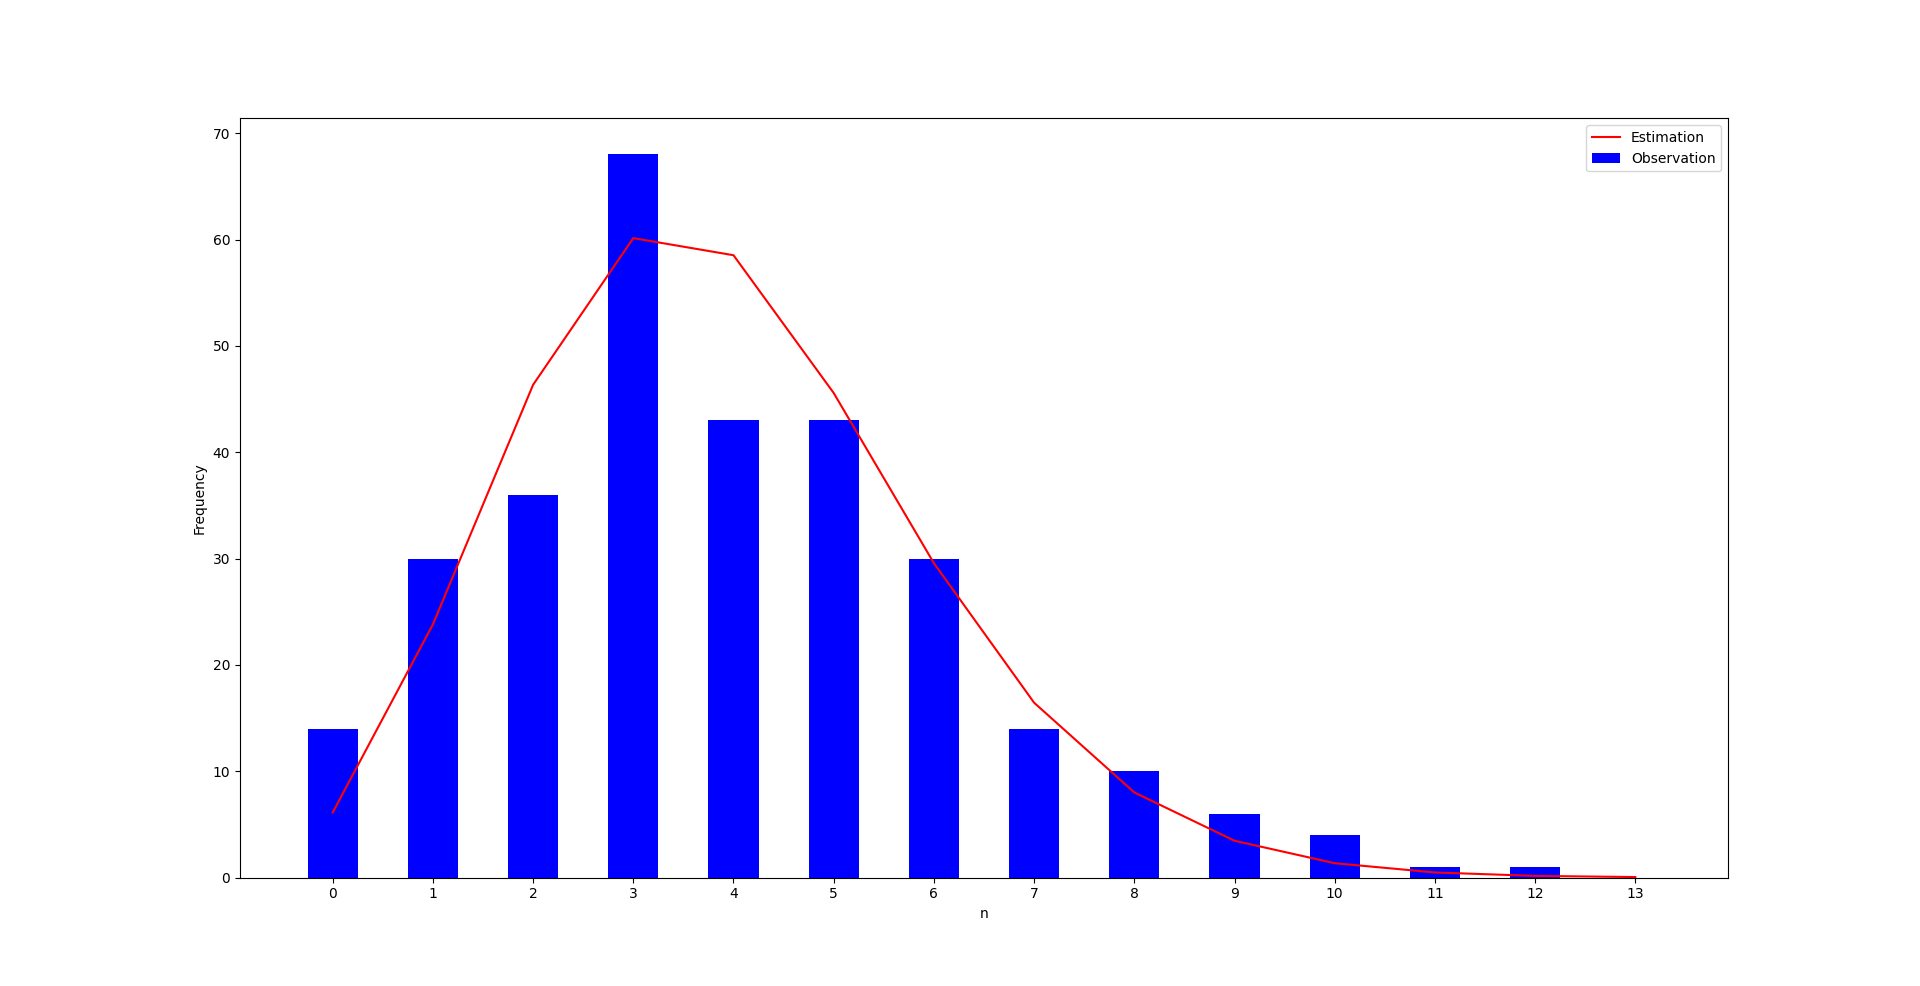
\includegraphics[width=10cm, height=10cm]{fig.jpeg}
       \caption{Analysis of Sorting Algorithms}
       \label{fig:my_label}
   \end{figure}
  \end{solution}


\end{questions}
\end{document}

%%% Local Variables:
%%% mode: latex
%%% TeX-master: t
%%% End:
